\section{Risultati}\label{sec:risultati}
Le misure sono state svolte sotto le condizioni riportate in tabella \ref{tab:livelli-logici}.
I risultati dei test delle porte logiche sono riportati di seguente, nelle tabelle \ref{tab:and1-multiplexer}, \ref{tab:and2-multiplexer}, \ref{tab:or-multiplexer} e \ref{tab:not-multiplexer}.
I risultati delle misure del multiplexer in regime stazionario sono riportati in tabella \ref{tab:multiplexer}.
I risultati qualitativi del multiplexer in regime dinamico sono riportati in figura \ref{fig:multiplexer-wave}.


\begin{table}[H]
  \centering
  \begin{subtable}[H]{0.5\textwidth}
    \centering
    \begin{tabular}[t]{c  c | c  c | c  c}
      \hline
      A & B & V(A) & V(B) & Out & V(Out) (V)\\
      \hline
      0 & 0 & $V_{0}$ & $V_{0}$ & 0 & $0.222 \pm 0.002$ \\
      0 & 1 & $V_{0}$ & $V_{1}$ & 0 & $0.222 \pm 0.002$ \\
      1 & 0 & $V_{1}$ & $V_{0}$ & 0 & $0.223 \pm 0.002$ \\
      1 & 1 & $V_{1}$ & $V_{1}$ & 1 & $3.64 \pm 0.02$ \\
      \hline
    \end{tabular}
  \end{subtable}

  \vspace{.5cm}

  \begin{subtable}[H]{0.5\textwidth}
    \centering
    \begin{tabular}[t]{c  c | c  c | c  c}
      \hline
      A & B & V(A) & V(B) & Out & V(Out) (V)\\
      \hline
      0 & 0 & $V_{0}$ & $V_{0}$ & 0 & $0.218 \pm 0.002$ \\
      0 & 1 & $V_{0}$ & $V_{1}$ & 0 & $0.219 \pm 0.002$ \\
      1 & 0 & $V_{1}$ & $V_{0}$ & 0 & $0.219 \pm 0.002$ \\
      1 & 1 & $V_{1}$ & $V_{1}$ & 1 & $3.64 \pm 0.02$ \\
      \hline
    \end{tabular}
  \end{subtable}

  \vspace{.5mm}

\begin{subtable}[H]{0.5\textwidth}
    \centering
    \begin{tabular}[t]{c  c | c  c | c  c}
      \hline
      A & B & V(A) & V(B) & Out & V(Out) (V)\\
      \hline
      0 & 0 & $V_{0}$ & $V_{0}$ & 0 & $0.223 \pm 0.002$ \\
      0 & 1 & $V_{0}$ & $V_{1}$ & 0 & $0.223 \pm 0.002$ \\
      1 & 0 & $V_{1}$ & $V_{0}$ & 0 & $0.223 \pm 0.002$ \\
      1 & 1 & $V_{1}$ & $V_{1}$ & 1 & $3.64 \pm 0.02$ \\
      \hline
    \end{tabular}
  \end{subtable}

  \vspace{.5cm}

  \begin{subtable}[H]{0.5\textwidth}
    \centering
    \begin{tabular}[t]{c  c | c  c | c  c}
      \hline
      A & B & V(A) & V(B) & Out & V(Out) (V)\\
      \hline
      0 & 0 & $V_{0}$ & $V_{0}$ & 0 & $0.217 \pm 0.002$ \\
      0 & 1 & $V_{0}$ & $V_{1}$ & 0 & $0.217 \pm 0.002$ \\
      1 & 0 & $V_{1}$ & $V_{0}$ & 0 & $0.217 \pm 0.002$ \\
      1 & 1 & $V_{1}$ & $V_{1}$ & 1 & $3.64 \pm 0.02$ \\
      \hline
    \end{tabular}
  \end{subtable}
  
  \caption{\emph{Tavole di verità delle porte \textsc{and} corrispondenti ai pin 1-2-3, 4-5-6, 13-12-11, 10-9-8 dell'integrato 7408 (A). I valori di $V_{0}$ e $V_{1}$ sono quelli riportati in tabella \ref{tab:livelli-logici}}}
  \label{tab:and1-multiplexer}
\end{table}

\begin{table}[H]
  \centering
\begin{subtable}[H]{0.5\textwidth}
    \centering
    \begin{tabular}[t]{c  c | c  c | c  c}
      \hline
      A & B & V(A) & V(B) & Out & V(Out) (V)\\
      \hline
      0 & 0 & $V_{0}$ & $V_{0}$ & 0 & $0.128 \pm 0.002$ \\
      0 & 1 & $V_{0}$ & $V_{1}$ & 0 & $0.129 \pm 0.002$ \\
      1 & 0 & $V_{1}$ & $V_{0}$ & 0 & $0.131 \pm 0.002$ \\
      1 & 1 & $V_{1}$ & $V_{1}$ & 1 & $4.41 \pm 0.02$ \\
      \hline
    \end{tabular}
  \end{subtable}

  \vspace{.5cm}

  \begin{subtable}[H]{0.5\textwidth}
    \centering
    \begin{tabular}[t]{c  c | c  c | c  c}
      \hline
      A & B & V(A) & V(B) & Out & V(Out) (V)\\
      \hline
      0 & 0 & $V_{0}$ & $V_{0}$ & 0 & $0.129 \pm 0.002$ \\
      0 & 1 & $V_{0}$ & $V_{1}$ & 0 & $0.129 \pm 0.002$ \\
      1 & 0 & $V_{1}$ & $V_{0}$ & 0 & $0.129 \pm 0.002$ \\
      1 & 1 & $V_{1}$ & $V_{1}$ & 1 & $4.41 \pm 0.02$ \\
      \hline
    \end{tabular}
  \end{subtable}
  
  

  \vspace{.5mm}

  \begin{subtable}[H]{0.5\textwidth}
    \centering
    \begin{tabular}[t]{c  c | c  c | c  c}
      \hline
      A & B & V(A) & V(B) & Out & V(Out) (V)\\
      \hline
      0 & 0 & $V_{0}$ & $V_{0}$ & 0 & $0.130 \pm 0.002$ \\
      0 & 1 & $V_{0}$ & $V_{1}$ & 0 & $0.130 \pm 0.002$ \\
      1 & 0 & $V_{1}$ & $V_{0}$ & 0 & $0.129 \pm 0.002$ \\
      1 & 1 & $V_{1}$ & $V_{1}$ & 1 & $4.39 \pm 0.02$ \\
      \hline
    \end{tabular}
  \end{subtable}

  \vspace{.5cm}
  
  \begin{subtable}[H]{0.5\textwidth}
    \centering
    \begin{tabular}[t]{c  c | c  c | c  c}
      \hline
      A & B & V(A) & V(B) & Out & V(Out) (V)\\
      \hline
      0 & 0 & $V_{0}$ & $V_{0}$ & 0 & $0.129 \pm 0.002$ \\
      0 & 1 & $V_{0}$ & $V_{1}$ & 0 & $0.129 \pm 0.002$ \\
      1 & 0 & $V_{1}$ & $V_{0}$ & 0 & $0.129 \pm 0.002$ \\
      1 & 1 & $V_{1}$ & $V_{1}$ & 1 & $4.40 \pm 0.02$ \\
      \hline
    \end{tabular}
  \end{subtable}
  \caption{\emph{Tavole di verità delle porte \textsc{and} corrispondenti ai pin 1-2-3, 4-5-6, 13-12-11, 10-9-8 dell'integrato 7408 (B). I valori di $V_{0}$ e $V_{1}$ sono quelli riportati in tabella \ref{tab:livelli-logici}}}
  \label{tab:and2-multiplexer}
\end{table}

\begin{table}[H]
  \centering
\begin{subtable}[H]{0.5\textwidth}
    \centering
    \begin{tabular}[t]{c  c | c  c | c  c}
      \hline
      A & B & V(A) & V(B) & Out & V(Out) (V)\\
      \hline
    0 & 0 & $V_{0}$ & $V_{0}$ & 0 & $0.066 \pm 0.002$ \\
    0 & 1 & $V_{0}$ & $V_{1}$ & 1 & $4.07  \pm 0.02$ \\
    1 & 0 & $V_{1}$ & $V_{0}$ & 1 & $4.07  \pm 0.02$ \\
    1 & 1 & $V_{1}$ & $V_{1}$ & 1 & $4.07 \pm 0.02$ \\
      \hline
    \end{tabular}
  \end{subtable}

  \vspace{.5cm}

  \begin{subtable}[H]{0.5\textwidth}
    \centering
    \begin{tabular}[t]{c  c | c  c | c  c}
      \hline
      A & B & V(A) & V(B) & Out & V(Out) (V)\\
      \hline
    0 & 0 & $V_{0}$ & $V_{0}$ & 0 & $0.071 \pm 0.002$ \\
    0 & 1 & $V_{0}$ & $V_{1}$ & 1 & $4.07  \pm 0.02$ \\
    1 & 0 & $V_{1}$ & $V_{0}$ & 1 & $4.07  \pm 0.02$ \\
    1 & 1 & $V_{1}$ & $V_{1}$ & 1 & $4.06 \pm 0.02$ \\
      \hline
    \end{tabular}
  \end{subtable}

  \vspace{.5mm}

  \begin{subtable}[H]{0.5\textwidth}
    \centering
    \begin{tabular}[t]{c  c | c  c | c  c}
      \hline
      A & B & V(A) & V(B) & Out & V(Out) (V)\\
      \hline
   0 & 0 & $V_{0}$ & $V_{0}$ & 0 & $0.072  \pm 0.002$ \\
    0 & 1 & $V_{0}$ & $V_{1}$ & 1 & $4.06  \pm 0.02$ \\
    1 & 0 & $V_{1}$ & $V_{0}$ & 1 & $4.06  \pm 0.02$ \\
    1 & 1 & $V_{1}$ & $V_{1}$ & 1 & $4.06 \pm 0.02$ \\
      \hline
    \end{tabular}
  \end{subtable}

  \caption{\emph{Tavole di verità delle porte \textsc{or} corrispondenti ai pin 1-2-3, 4-5-6, 13-12-11 dell'integrato 7432. I valori di $V_{0}$ e $V_{1}$ sono quelli riportati in tabella \ref{tab:livelli-logici}}.}
  \label{tab:or-multiplexer}
\end{table}




\begin{table}[H]
  \centering
\begin{subtable}[H]{0.5\textwidth}
    \centering
        \begin{tabular}[t]{c  c | c  c }
      \hline
      A & V(A) & Out & V(Out) (V) \\
      \hline
          0 & $V_{0}$ & 1 & $4.39 \pm 0.02$ \\
      1& $V_{1}$ & 0 & $0.108 \pm 0.002$ \\
      \hline
    \end{tabular}
  \end{subtable}

  \vspace{.5cm}

  \begin{subtable}[H]{0.5\textwidth}
    \centering
        \begin{tabular}[t]{c  c | c  c }
      \hline
      A & V(A) & Out & V(Out) (V) \\
      \hline
      0 & $V_{0}$ & 1 & $4.39 \pm 0.02$ \\
      1& $V_{1}$ & 0 & $0.109 \pm 0.002$ \\
      \hline
    \end{tabular}
  \end{subtable}

  \caption{\emph{Tavole di verità delle porte \emph{not} corrisponenti ai pin 1-2, 3-4 dell'integrato 7404. I valori di $V_{0}$ e $V_{1}$ sono quelli riportati in tabella \ref{tab:livelli-logici}}.}
  \label{tab:not-multiplexer}
\end{table}


\begin{table}[H]
  \centering
  \begin{tabular}{c c | c c | c c }
    \hline
    $I_{1}$ & $I_{0}$ & $S_{1}$ & $S_{0}$ & Out & V(Out) (V) \\
    \hline
    1 & 0 & 0 & 0 & 0 & $0.0776 \pm 0.0001$ \\
    0 & 1 & 0 & 0 & 1 & $3.85 \pm 0.02$ \\
    0 & 1 & 0 & 1 & 0 & $0.0790 \pm 0.0003$ \\
    1 & 0 & 0 & 1 & 1 & $3.87 \pm 0.02$ \\
    1 & 1 & 1 & 0 & 0 & $0.0793 \pm 0.0003$ \\
    0 & 0 & 1 & 0 & 1 & $3.78 \pm 0.02$ \\
    1 & 1 & 1 & 1 & 0 & $0.0794 \pm 0.0003$ \\
    0 & 0 & 1 & 1 & 1 & $3.76 \pm 0.02$ \\
  \end{tabular}
  \caption{\emph{Tavola di verità del multiplexer.}}
  \label{tab:multiplexer}
\end{table}

\begin{figure}[H]
   \centering
        \centering
        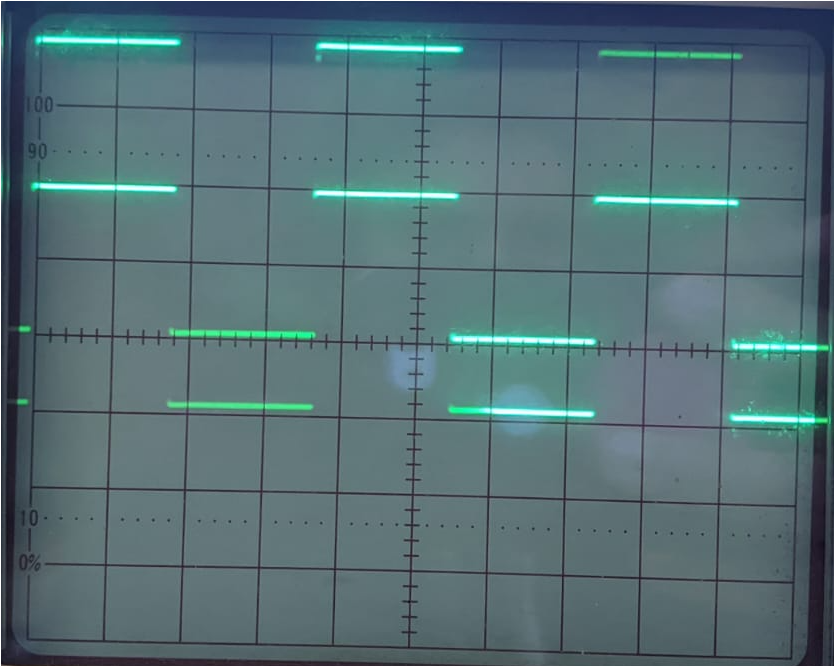
\includegraphics[width=10cm]{../assets/sinusoide.png}
        \caption{\emph{Risposta del multiplexer quando in un input è presente un onda quadra e quello stesso input è selezionato come output.}}
    \label{fig:multiplexer-wave}
  \end{figure}